\section{Evaluation}
\label{sec:evalation}

In this section, we evaluate various aspects of DTRIM and compare it with the conventional translation.

\begin{comment}
\begin{figure*}[t]
	\centering
	\subfloat[Hash Table]{
		\label{fig:memcached_2p_assoc}
		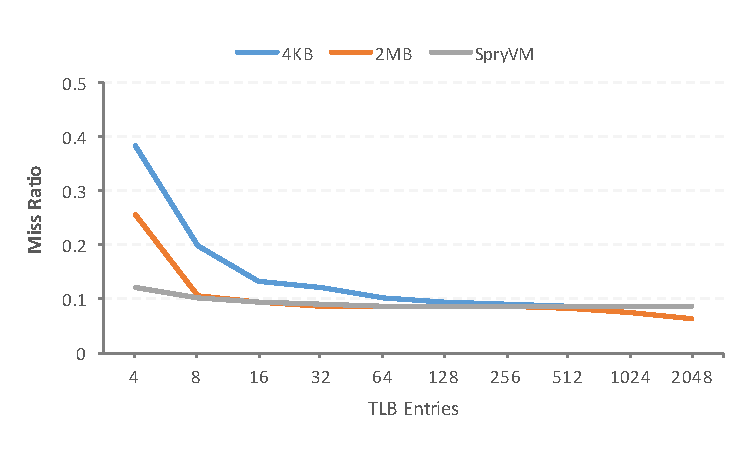
\includegraphics[width=0.3\textwidth,clip]{graphs/HT_32GB.pdf}}
	\subfloat[Skip List]{
		\label{fig:memcached_4p_assoc}
		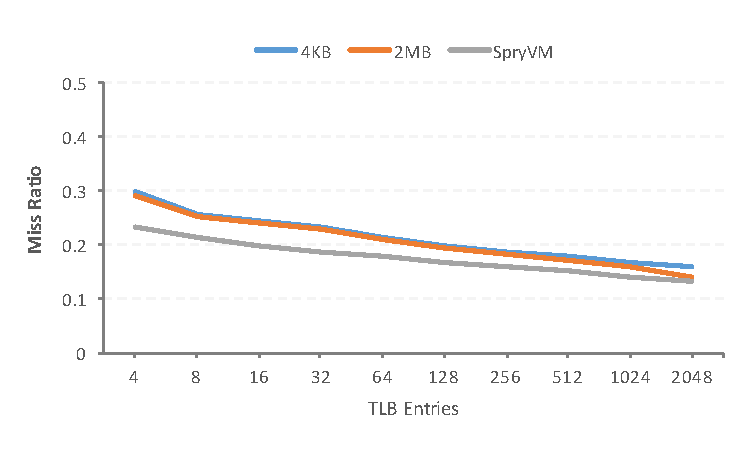
\includegraphics[width=0.3\textwidth,clip]{graphs/SL_32GB.pdf}}
	\hspace{.01in}
	\subfloat[BST Internal]{
		\label{fig:rocksdb_2p}
		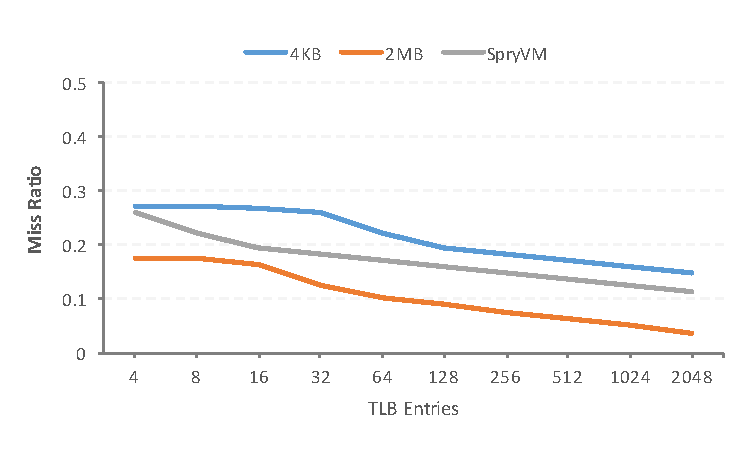
\includegraphics[width=0.3\textwidth,clip]{graphs/BSTI_32GB.pdf}}
	\subfloat[BST External]{
		\label{fig:rocksdb_4p}
		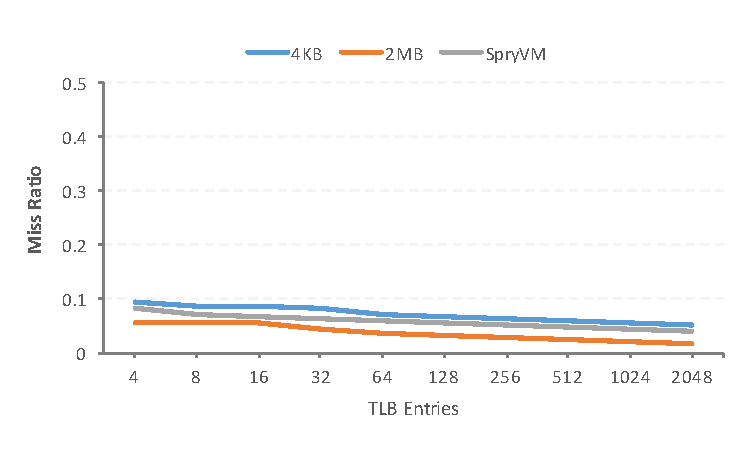
\includegraphics[width=0.3\textwidth,clip]{graphs/BSTE_32GB.pdf}}

	
	\caption{TLB sensitivity study for 32GB working set for conventional translation with 4KB and 2MB pages and DTRIM.
		\label{fig:miss_ratio_32GB}}
\end{figure*}

\begin{figure*}[t]
	\centering
	\subfloat[Hash Table]{
		\label{fig:memcached_2p_assoc}
		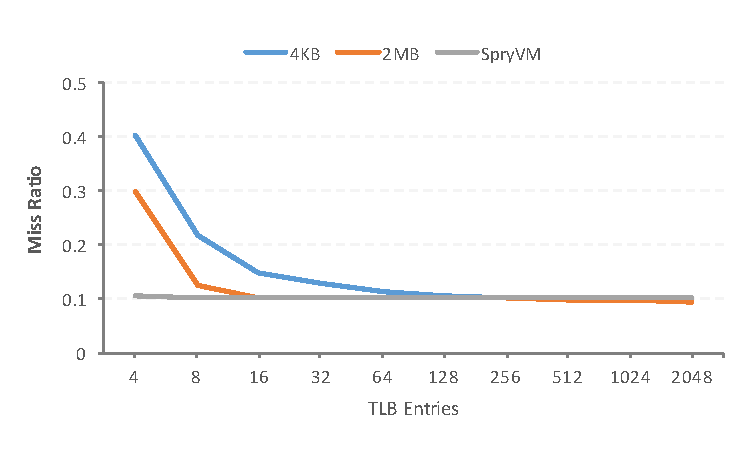
\includegraphics[width=0.3\textwidth,clip]{graphs/HT_128GB.pdf}}
	\subfloat[Skip List]{
		\label{fig:memcached_4p_assoc}
		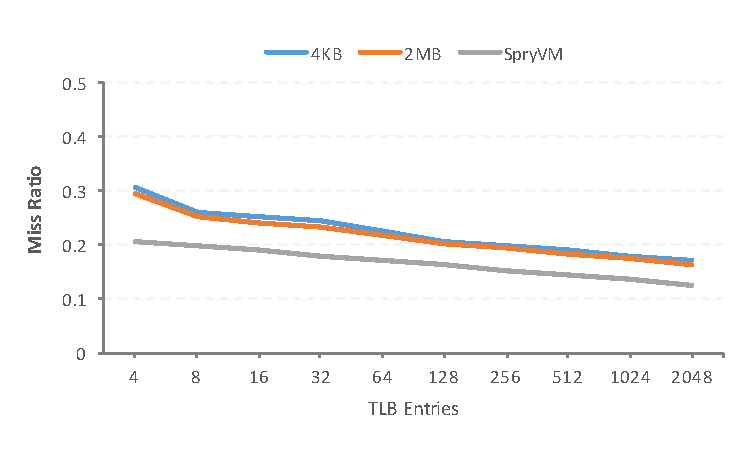
\includegraphics[width=0.3\textwidth,clip]{graphs/SL_128GB.pdf}}
	\hspace{.01in}
	\subfloat[BST Internal]{
		\label{fig:rocksdb_2p}
		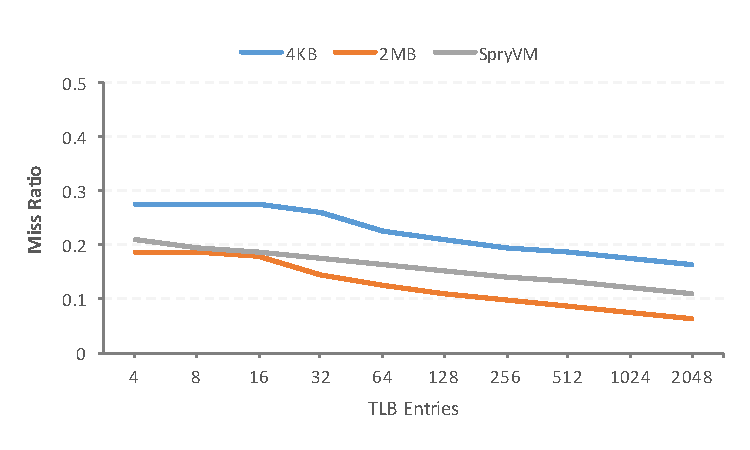
\includegraphics[width=0.3\textwidth,clip]{graphs/BSTI_128GB.pdf}}
	\subfloat[BST External]{
		\label{fig:rocksdb_4p}
		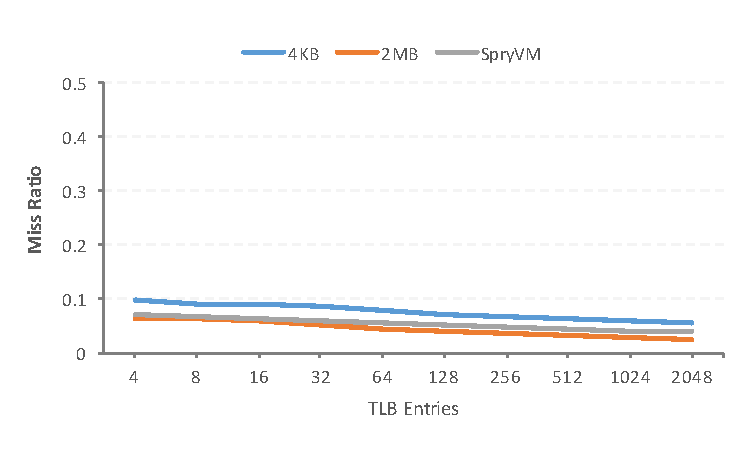
\includegraphics[width=0.3\textwidth,clip]{graphs/BSTE_128GB.pdf}}
	
	
	\caption{TLB sensitivity study for 128GB working set for conventional translation with 4KB and 2MB pages and DTRIM.
		\label{fig:miss_ratio_128GB}}
\end{figure*}

\subsection{TLB Sensitivity}
~\subsubsection{32GB working set.} Figure~\ref{fig:miss_ratio_32GB} shows the TLB miss ratio as we increase the number of entries, of the four data structure traversals, hash table, skip list, binary search tree internal, and binary search tree external, with a working set size of $32$GBs. Each graph plots three lines. The blue line represents the conventional translation mechanism using 4KB pages. The orange line the same mechanism but using $2$MB pages. The gray bar represent the TLB miss ratio of DTRIM, which uses $4$KB pages.

\noindent\textbf{4KB pages:} For all four data structures, DTRIM
systematically beats conventional translation with $4$KB pages given
the same TLB size. For example, for the hash table, conventional
translation requires a 128-entry TLB to match the miss ratio of DTRIM
with 8 entries, a $16\times$ difference. Furthermore, we see that the
gap between the efficiency of TLBs worsens with the absence of data
locality. For the skip list, which is the workload with the lowest
data locality, conventional translation requires around $2048$ entries
to match the miss ratio of DTRIM with 16 entries.

\noindent\textbf{2MB pages:} Using $2$MB pages improves the TLB
behavior of conventional translation. For example, for the hash table,
with 2MB pages, conventional translation only need 8 entries to match
the miss ratio of 4 entries in DTRIM, a $2\times difference$. In
contrast, in workloads where there exist data locality, like in the
trees, in which there is data reuse for the higher levels of the tree,
the per-region $4KB$ pages are not able to beat $2$MB pages. However,
note that $2$MB are not always available (as explained in the
background section) and we could also employ $2MB$ pages for DTRIM;
we defer that approach for future work. Furthermore, in workloads
where there exists no locality, such as in the skip list data
structure, $2$MB deliver an almost negligible improvement with respect
to $4KB$ pages (also shown in prior work for other data structure with
low data locality like graphs~\cite{haria:devirtualizing}). Hence, for
the skip list, the number of TLB entries still needs to be $16\times$
bigger to match DTRIM's TLB area efficiency.

~\subsubsection{128GB working set.} Figure~\ref{fig:miss_ratio_128GB}
shows the TLB miss ratio as we increase the number of entries of the
four data structure traversals with a working set size of
$128$GBs. Similarly to the previous set of graphs, each graph plots
three lines: conventional translation with 4KB pages, the same
mechanism but using $2$MB pages, and SryVM, which uses $4$KB pages.

\noindent\textbf{4KB pages:} For all four data structures, DTRIM
systematically beats conventional translation with $4$KB pages given
the same TLB size. Furthermore, the area-efficiency gap is more
pronounced as the working set is larger.

\noindent\textbf{2MB pages:} Although $2$MB pages helps to reduce the
area-efficiency gap with respect to $4$KB and DTRIM, the increase in
the working set worses the benefits. For example, in the hash table,
$2$MB pages now requires $8\times$ the number of TLB entries to match
the miss ratio of 4 TLB entries in DTRIM. Furthermore, in the cases
where there is more data locality, the situation also worsens, and in
fact, for the binary search tree external, now $2$MB pages and DTRIM,
behave almost identically.
\end{comment}

\begin{figure*}[t]
    \centering
    \subfloat{
        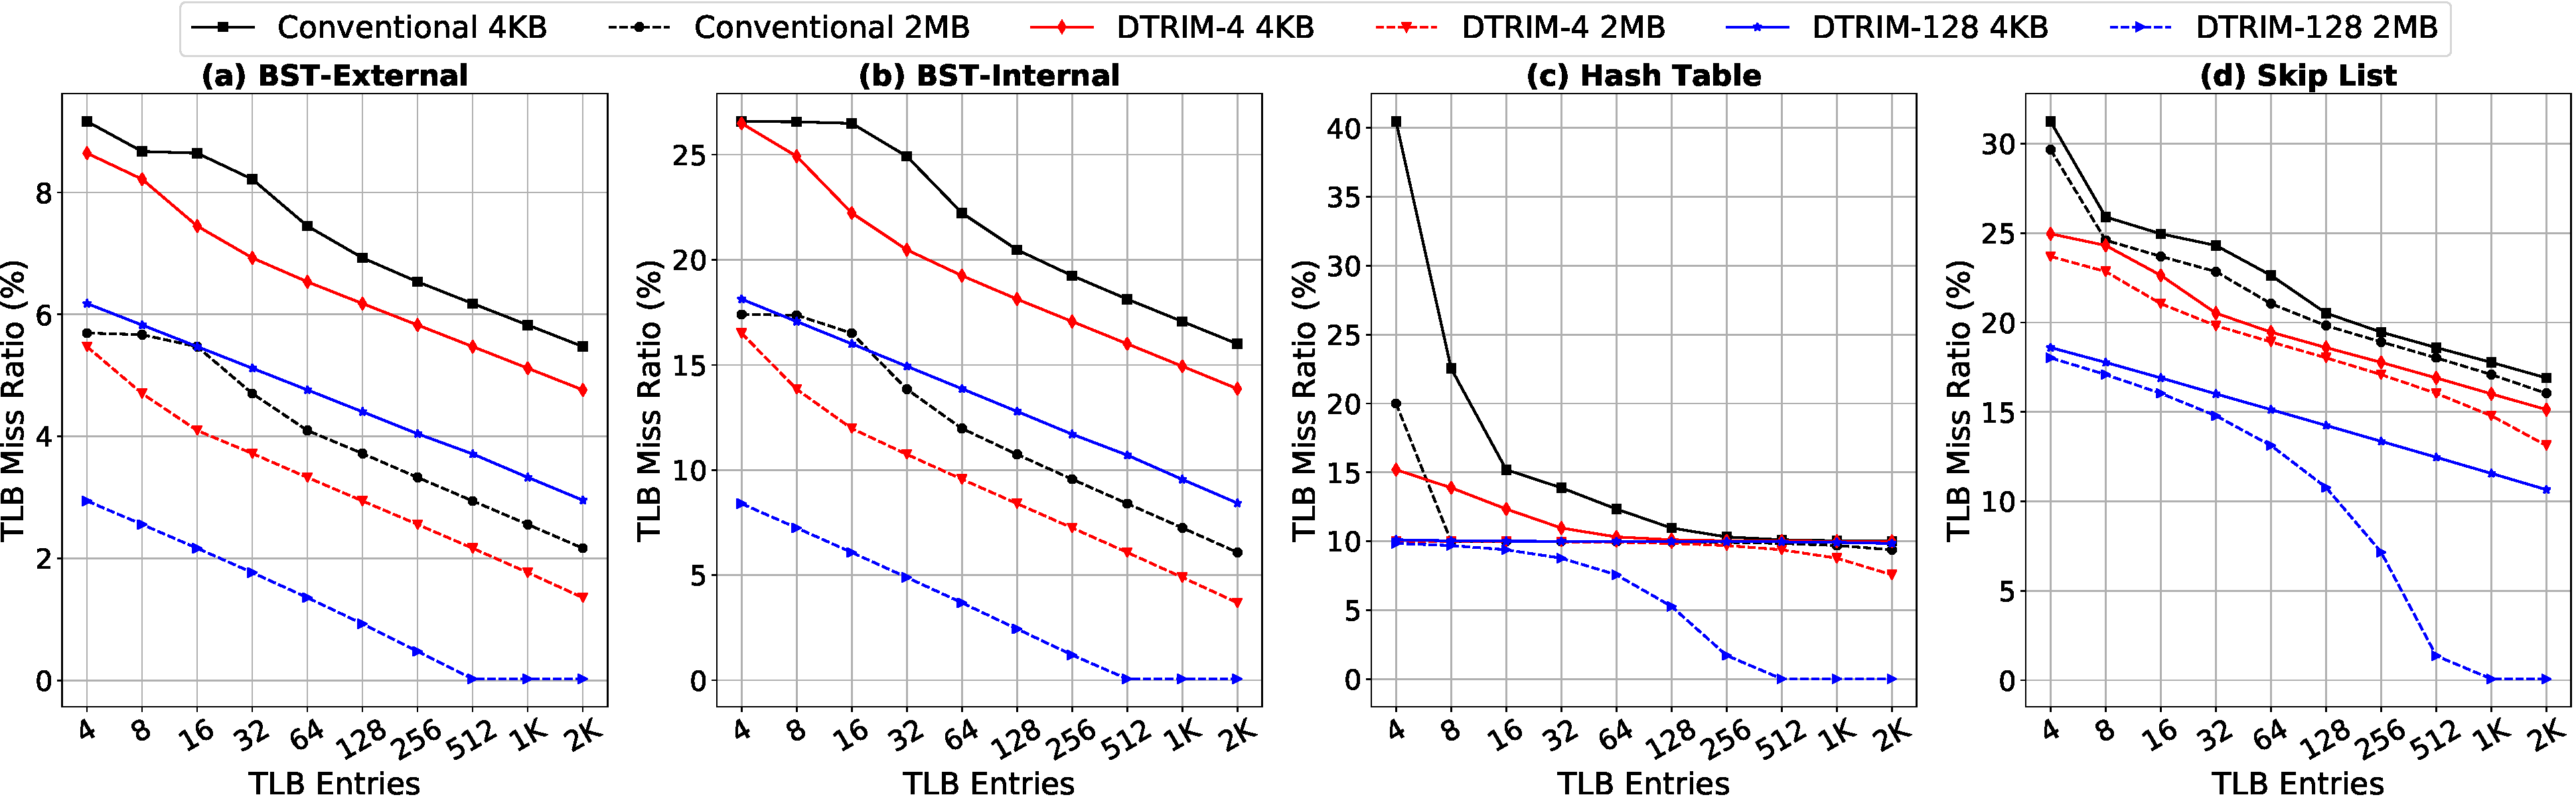
\includegraphics[width=1 \textwidth,clip]{graphs/all_128G_entries.pdf}}
    \caption{TLB sensitivity study for 128GB working set for conventional translation with 4KB and 2MB pages and DTRIM.}
    \label{fig:miss_ratio_128GB}
\end{figure*}


\subsection{TLB Sensitivity}
Figure~\ref{fig:miss_ratio_128GB} shows the TLB miss ratio for the four data traversal benchmarks: hash table, skip lists, internal and external binary search trees, as we vary the number of TLB entries. The working set size of all workloads is $128$GBs, and the TLB associativity is fixed to 4 ways. Each graph plots six lines. The full black line shows the TLB miss ratio for the conventional translation with 4KB pages, while the dotted black line shows the TLB miss ratio for conventional translation with 2MB pages. The red lines show TLB miss ratio for DTRIM, assuming only four memory partitions; the full red line shows the DTRIM with 4KB pages, while the dotted red line shows DTRIM with 2MB pages. It is important to note that the use of huge pages is orthogonal and fully compatible with our approach. Finally, the blue lines show the TLB miss ratio for DTRIM with 128 memory partitions, with the full blue lines showing the case with 4KB pages, and blue dotted lines showing the case with 2MB pages. 

For all workloads, the DTRIM configuration with only 4 memory partitions (full red line) significantly outperforms the conventional translation with 4KB pages (full black line). On average, the memory-side TLB require about 4x fewer TLB entries to match the performance of conventional execution-side TLBs. This efficiency of memory-side TLBs is attributed to their distributed nature: they cover only a fraction of the physical memory space. As expected, conventional TLBs with 2MB pages (black dotted line) perform strictly better compared to the TLBs with 4KB page sizes (full black line), often outperforming the DTRIM configuration with 4KB pages (red full line) as well. However, for some workloads with poor spatial locality, such as skip lists, the memory-side TLBs with 4KB pages (full red line) are even able to outperform conventional TLBs with 2MB pages (black dotted line) with the same number of entries. 

DTRIM is not bound to any page size and can be implemented with 2MB pages as well. Red dotted line shows TLB miss ratio with 2MB pages for DTRIM with 4 partitions. Not surprisingly, this configuration greatly outperforms the conventional designs with both 4KB and 2MB pages, as well as the DTRIM configuration with 4KB pages. An interesting case is the DTRIM configuration with 128 partitions and 4KB pages (full blue line). It outperforms all other configurations with 4KB pages, but also the configurations with 2MB pages for some workloads, such as skip lists. This shows that for workloads with low spatial locality, the benefits of further memory partitioning is much more significant than the impact of increasing the page size. However, the two techniques, partitioning and huge pages, are orthogonal and mutually compatible. Finally, the DTRIM configuration with 128 partitions and 2MB pages (blue dotted line) offers unmatched performance. With only 4 entries this configuration is able to outperform the conventional configurations with 2048 TLB entries for most of the workloads and page sizes.

\subsection{TLB Miss Penalty}

DTRIM does not only improve the area-efficiency of TLBs but also reduces the TLB miss penalty. Figure~\ref{fig:penalty} shows the TLB miss penalty of a memory reference, including the data access to memory, normalized to the ideal translation mechanism where only the data access of the memory references is required. We decided to be conservative and assume perfect MMU caches, and therefore page walks requires only one memory reference. The reason is because we want to decouple the TLB miss penalty benefits from the page table implementation, since in our case, with an inverted page table of $1/4x$ of load factor, we are able to guarantee one memory reference per page walk, whereas the hierarchical four-level page table requires a very significant MMU cache hierarchy. Furthermore, we consider two systems, a conventional two-socket machine and a large-memory eight-socket machine.

As the figure shows, page walks in a conventional VM mechanism requires a memory reference to locate the page table entry, and hence a memory reference requires two memory accesses. In contrast, and as explain in Figure~\ref{fig:pagewalk_partition_miss}, the virtual address uniquely identifies the memory region, and hence the time it takes to locate the region, traversing the NoC and off-chip interconnects is overlapped with the data path. Furthermore, the larger the memory systems, the larger the contribution of the network time in the page walk time, and hence the large the reduction in page walk time with respect with conventional translation. 

\begin{figure}[t]
	\centering
	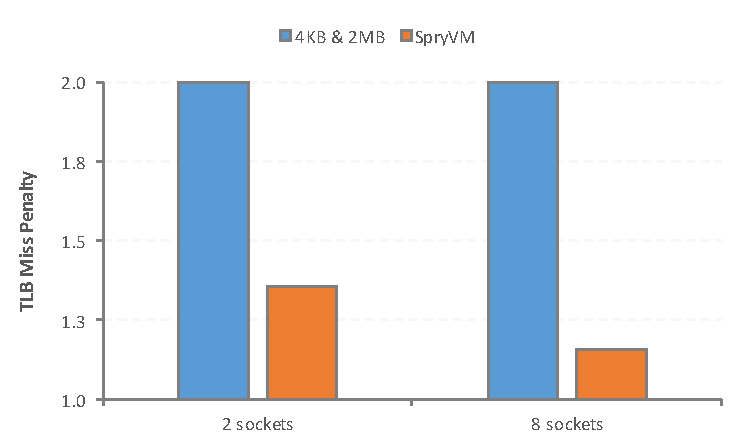
\includegraphics[width=0.8\columnwidth]{graphs/penalty.pdf}
	\caption{TLB miss penalty for conventional and DTRIM.}
	\label{fig:penalty}
\end{figure}

\subsection{Thread Contention}


\begin{figure*}[t]
    \centering
    \subfloat{
        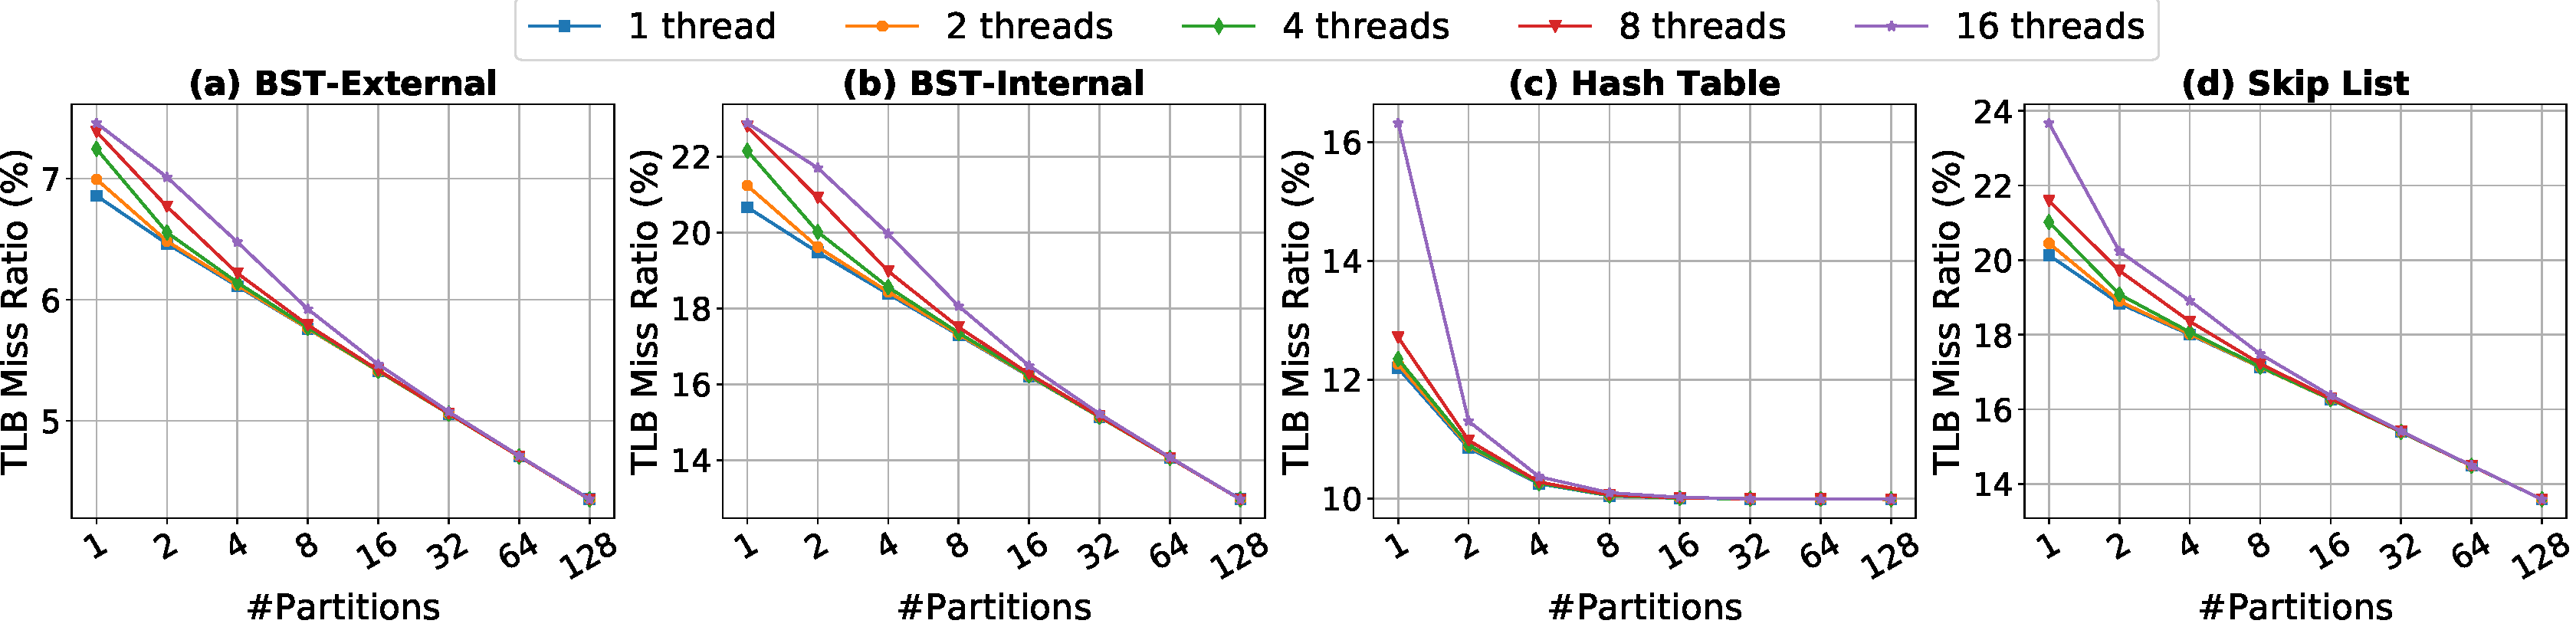
\includegraphics[width=1 \textwidth,clip]{graphs/multithreading.pdf}}
    \caption{The impact of thread contention on TLB miss rates.}
    \label{fig:contention}
\end{figure*}


Partitioning of the physical address space through set-associativity enables effective memory-side address translation with significantly reduced TLB miss rates.  However, a major consequence moving the translation from the place of execution to the memory partitions is that the per-partition TLBs become shared by all threads in the system that are accessing a given partition. A large system with many cores and accelerators could have hundreds of threads, which can create two potential problems related to TLB contention, which do not exist in conventional TLBs. The first problem is the limited TLB bandwidth, and the second problem is the interference among threads. 

The first problem arises when TLBs cannot serve the volume of accesses generated by all threads. Fortunately, this problem does not occur in DTRIM. The reason is that even conventional TLBs are designed to sustain the L1 cache bandwidth of a single core, which is in the order of 100s of GB/s. In the case of DTRIM, the TLB bandwidth needs to be adequate to sustain the memory bandwidth of the local DRAM partition, which is an order of magnitude less. Furthermore, the size of memory partitions could arbitrarily reduced. The second problem arises when different threads compete for the limited capacity of the shared per-partition TLB. To quantify this problem, we measure the TLB miss rates in DTRIM while varying the number of threads and the number of memory partitions. The results are shown in Figure~\ref{fig:contention}. In this experiment, the memory footprint of all applications is 64GB, the size of TLBs is 128 entries, and their associativity is fixed to four. The first thing to notice is that, in the single-threaded case, the TLB miss rates drop dramatically with the number of partitions as a result of physical address space partitioning, corroborating our real hardware experiments in Figure~\ref{fig:pagewalks}. The next thing to notice is that, in the case of a single memory partition, most application exhibit a noticeable increase in TLB miss rates as we add more threads, as many threads contend for the capacity of a single shared TLB that covers the entire memory (a similar effect could be observed with hyper-threading, when multiple threads share the same TLB). However, once we start increasing the number of memory partitions, the impact of thread contention virtually disappears, showing that the benefits of partitioning significantly outweighs the impact of contention. This becomes most obvious when comparing (1 partition, 1 thread) and (16 partitions, 16 threads) data  points, because they have the same number of aggregate TLB entries per thread and the reduction in miss rates in entirely contributed to DTRIM's organization. 

\subsection{Associativity study of VM}

\begin{figure*}
	\centering
	\subfloat[Memcached --- 1 Process]{
		\label{fig:memcached_1p}
		%  \includegraphics[width=.32\textwidth,clip,trim = 18mm 213mm 117mm 20mm]{figs/eps/sim-rread-lat.eps}}
		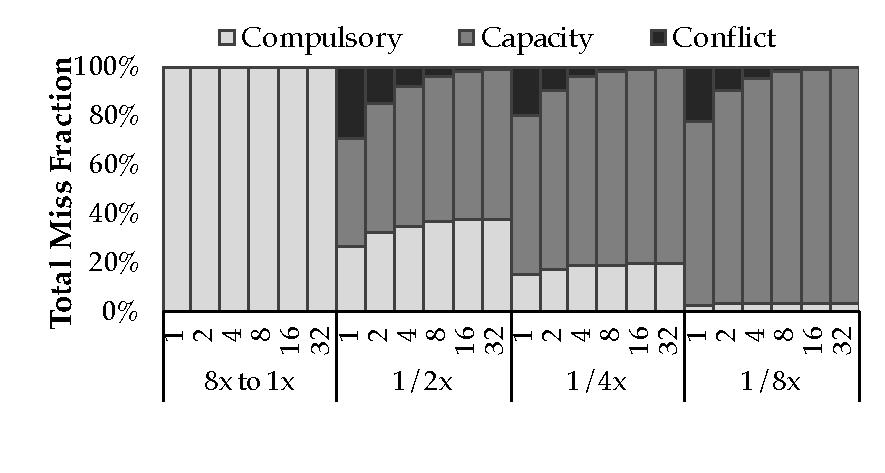
\includegraphics[width=.365\textwidth,clip]{graphs/memcached_assoc_1p-bw.pdf}}
	%  \hspace{.01in}
	\subfloat[RocksDB --- 1 Process]{
		\label{fig:rocksdb_1p}
		%  \includegraphics[width=.32\textwidth,clip,trim = 18mm 213mm 115mm 20mm]{figs/eps/sim-rread-bw.eps}}
		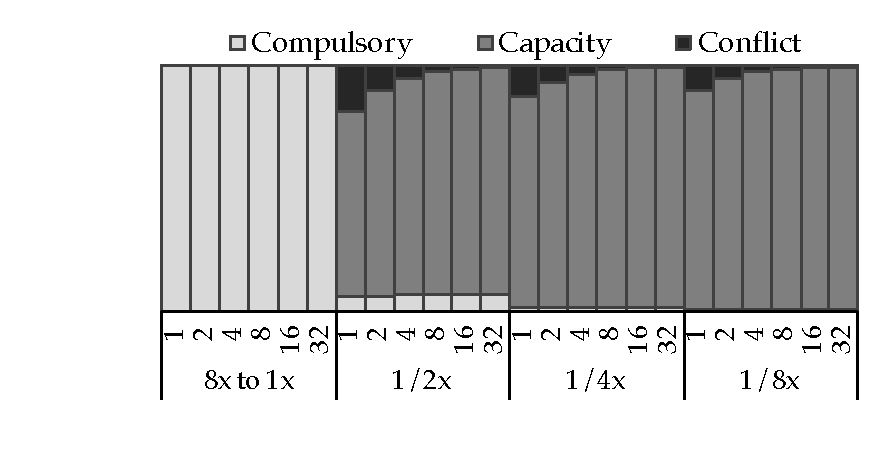
\includegraphics[width=.31\textwidth,clip]{graphs/rocksdb_assoc_1p-bw.pdf}}
	%   \hspace{.01in}
	\subfloat[Cassandra --- 1 Process]{
		\label{fig:cassandra_1p}
		%  \includegraphics[width=.32\textwidth,clip,trim = 28mm 217mm 115mm 20mm]{figs/eps/emu-rread-lat_cropped.eps}}
		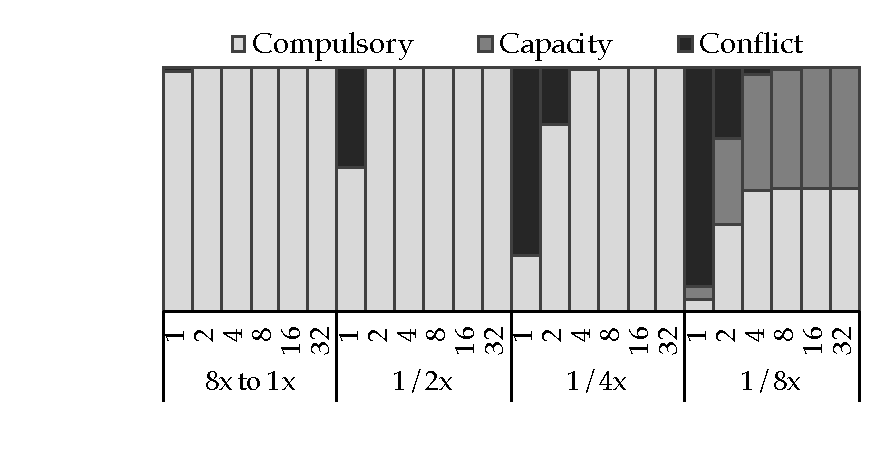
\includegraphics[width=.31\textwidth,clip]{graphs/cassandra_assoc_1p-bw.pdf}}
	\caption{Overall miss ratio broken down into compulsory, capacity, and conflict misses.
		\label{fig:miss_ratio}}
\end{figure*}

\begin{figure*}[t]
	\centering
	\subfloat[Memcached --- 2 Processes]{
		\label{fig:memcached_2p_assoc}
		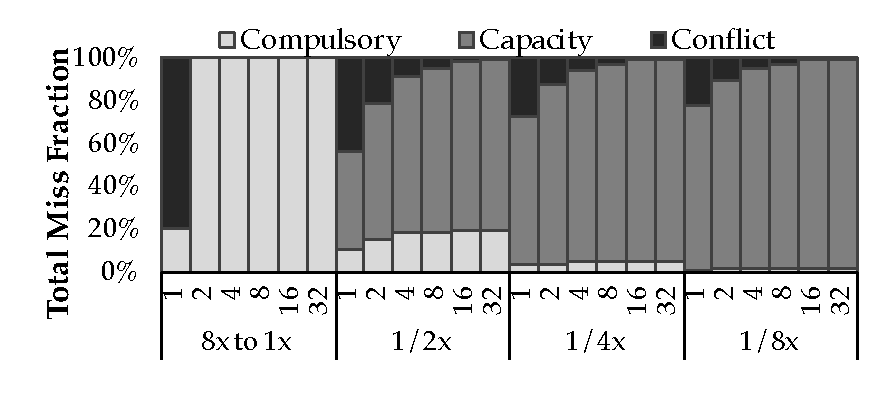
\includegraphics[width=.36\textwidth,clip]{graphs/memcached_assoc_2p-bw.pdf}}
	\subfloat[Memcached --- 4 Processes]{
		\label{fig:memcached_4p_assoc}
		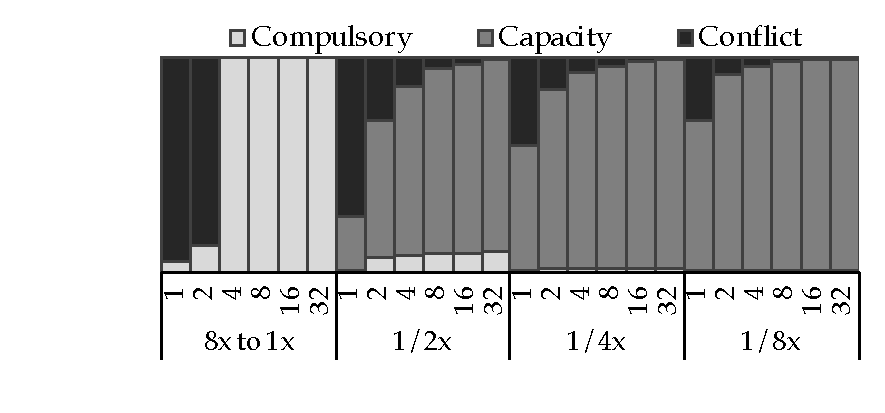
\includegraphics[width=.31\textwidth,clip]{graphs/memcached_assoc_4p-bw.pdf}}
	\subfloat[Memcached --- 8 Processes]{
		\label{fig:memcached_8p}
		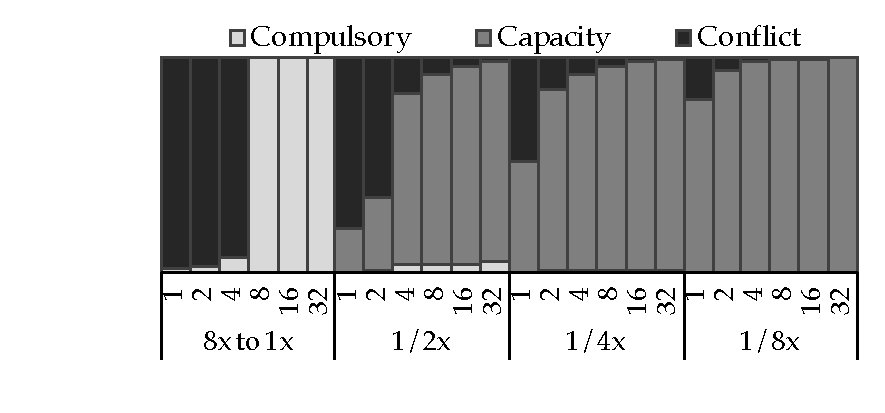
\includegraphics[width=.31\textwidth,clip]{graphs/memcached_assoc_8p-bw.pdf}}
	
	
	
	\caption{Overall miss ratio broken down into compulsory, capacity, and conflict misses.
		\label{fig:miss_ratio_procs}}
\end{figure*}

\subsection{Single-Process In-Memory}

Fig.~\ref{fig:miss_ratio} shows results for three single-process workloads: Memcached, RocksDB, and Cassandra. The y-axis breaks down the total misses into the three distinct miss classes. Each category on the x-axis corresponds to the ratio between the size of the physical memory and the size of the application's working set. For example,  $8\times$ indicates that the memory is eight times larger than the application's working set. Similarly, $1/2\times$ means that the application's working set is twice the size of the memory. We collapse results for $8\times$ to $1\times$ because they are similar and visually identical; each case represents a fully in-memory scenario. Furthermore, within each working set category, the x-axis sweeps through different VM associativities, from direct-mapped to 32-way associative. 



Even with a simple direct-mapped translation, compulsory misses represent $99.9\%$ of all the misses. There are no capacity misses as the working set fully fits in memory. Conflict misses are scarce. For example, Memcached using direct-mapped translation achieves a conflict miss rate in the order of one miss per $10^{8}$ memory accesses. Using $2$ ways removes all the conflicts for the $8\times$, $4\times$, and $2\times$ cases, while $4$ ways are required for the $1\times$ case (where the memory size is equal to izeablesize of the working set). For in-memory scenarios, page conflicts arise because the virtual address space of server applications is particularly sparse; there are many virtual segments scattered all over the address space. For example, Java processes exhibit many virtual segments due to the dynamic nature of the JVM. This is best observed in the case of Cassandra, which exhibits direct-mapped conflict miss rates in the order of one miss per $10^{7}$ and $10^{6}$ memory accesses for the $8\times$--$2\times$ cases and the $1\times$ case respectively. However, conflict misses drop rapidly as associativity increases and using 4 ways removes all conflicts for the $4\times$ and $2\times$ cases, while virtually eliminating conflicts for the $1\times$ case. The observation that conflict misses drop rapidly with associativity has also been shown for caches~\cite{hill:aspects, cantin:cache}. We elide the results for TPC-H, TPC-DS, and MySQL as they follow identical trends.

\subsection{Single-Process Out-of-Memory}

In contrast to in-memory scenarios, when the working sets do not fit in memory ($1/2\times$, $1/4\times$, $1/8\times$ cases), capacity misses grow with the working set size, while the fraction of compulsory misses drops. Although conflict misses are more significant than in the in-memory scenarios, conflicts drop sharply after 2-4 ways. In the worst case, 16 ways are required to drive conflict misses down to $\sim1\%$ of all the misses. Note that Cassandra has an active working set that fits in a memory of $1/4\times$ the data size, and capacity misses start to rise at the $1/8\times$ case and beyond. Fundamentally, all these results corroborate the seminal work on caches~\cite{hill:aspects, cantin:cache}. 

\subsection{Multi-programming In-Memory}
Fig.~\ref{fig:miss_ratio_procs} presents results for multi-programming. We take each of the three workloads, Memcached, RocksDB, and Cassandra, and increase the number of processes, keeping the overall working set size the same with respect to the single process scenarios. For example, for the $1\times$ case in Fig.~\ref{fig:miss_ratio}, the working set of a single process equals the size of the memory. In Fig.~\ref{fig:miss_ratio_procs}, for two processes sharing the same physical memory, the per-process working set is half the size of the physical memory. Similarly, with four processes, per-process working sets consume a quarter of the physical memory. We thus guarantee that only the increase in the number of processes has an impact on the associativity. 

For in-memory scenarios ($8\times$--$1\times$ cases), once the associativity equals the number of processes, compulsory misses represent $99.9\%$ of all the misses for all the workloads. Increasing the associativity further makes conflicts virtually disappear after a few additional ways. For instance, for Memcached, with 8, 16, and 32 ways, the conflicts are in the order of a single miss per $10^{9}$ accesses for 2, 4, and 8 processes, respectively. Cassandra requires 4, 8, and 8 ways to achieve a miss conflict rate of one miss per $10^{9}$ accesses for 2, 4, and 8 processes, respectively. Again, the trends are identical for TPC-H, TPC-DS, and MySQL. Overall, conflict misses become virtually zero with a few ways (i.e., 2-4) per process.

\subsection{Multi-programming Out-of-Memory}

For the cases where the working sets do not fit in memory, the trends are similar to the single-process scenarios. Capacity misses become more significant as the working set sizes grow, making conflict and compulsory misses less important. Similar to the in-memory case, once the associativity equals the number of processes, the fraction of conflict misses matches the single-process results. Conflicts drop rapidly as in the other cases and with 4 ways per process, conflict misses remain within $1\%$ of the total misses for all the workloads. The results for TPC-H, TPC-DS, and MySQL are identical.

\subsection{Linux Prototype}
\begin{figure}[t]
   \centering
   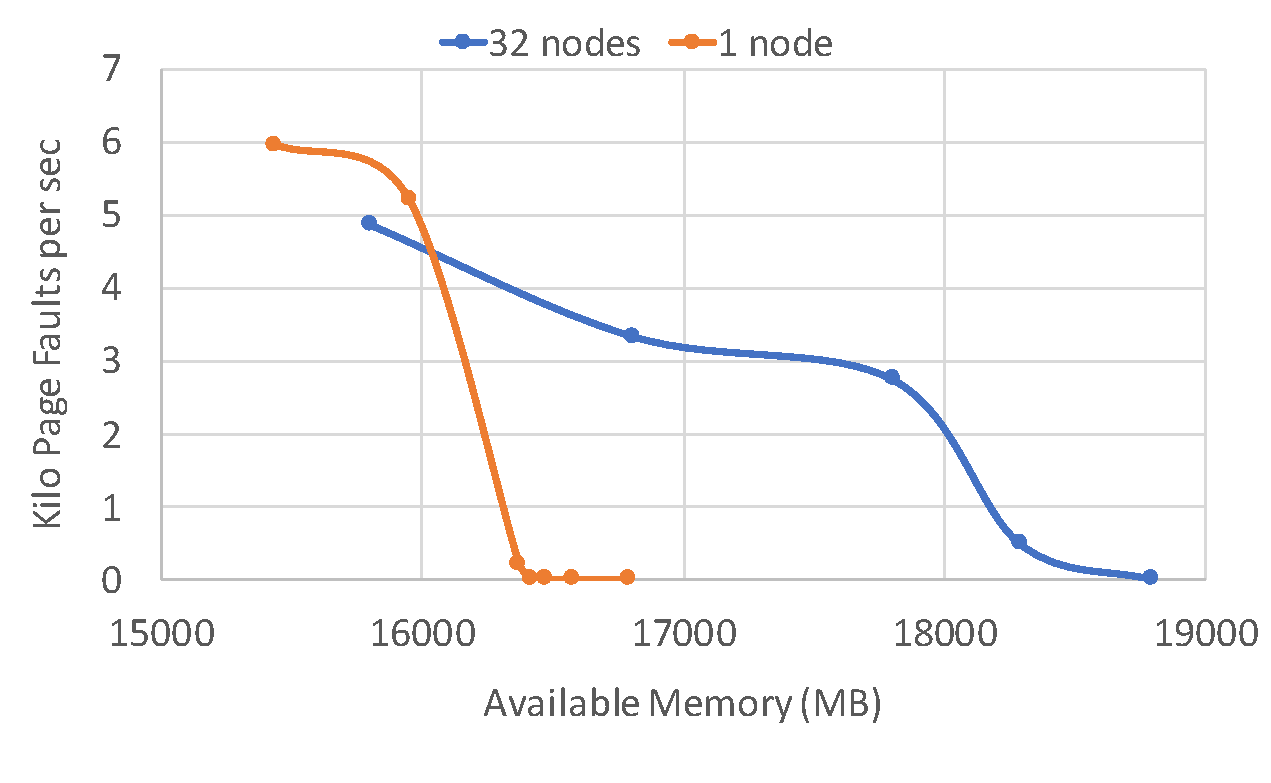
\includegraphics[width=1.0\columnwidth]{graphs/realhw.pdf}
   \caption{Page fault rate vs memory size for fully associative (1-node) and set-associative (32-nodes).}
   \label{fig:realhw}
\end{figure}


We successfully ran all server workloads on modified linux with 32 memory regions (nodes), utilizing above 90\% of available DRAM without a single page fault. Figure~\ref{fig:realhw} shows the page fault rate RocksDB tuned for a 16GB footprint, as we vary the available memory capacity in the critical range using the linux boot-time mem parameter. First, we note that our kernel properly deals with demand paging in the out-of-memory scenarios. Second, we see that the page fault rates in fully associative (1 partition) and set-associative (32 partitions) case follow the same trend, except that the 32-partition setup requires about 1.5--2GB more memory to achieve the same page-fault rate. We note that this is not related to associativity, given that the associativity reduction is minor. Instead, this effect is the artifact of the prototype that relies on linux NUMA nodes, which have small memory overheads per node and exhibit a degree of variability in their capacity. 

\begin{figure}[t]
	\centering
	\subfloat[32GB]{
		\label{fig:memcached_2p_assoc}
		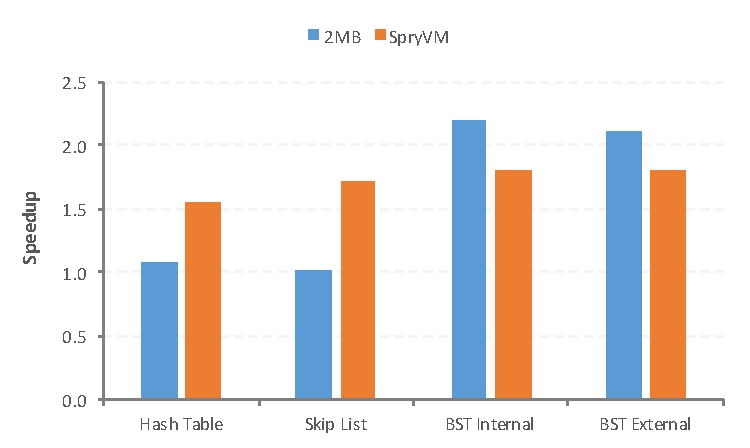
\includegraphics[width=0.25\textwidth,clip]{graphs/speedup_32GB.pdf}}
	\subfloat[128GB]{
		\label{fig:memcached_4p_assoc}
		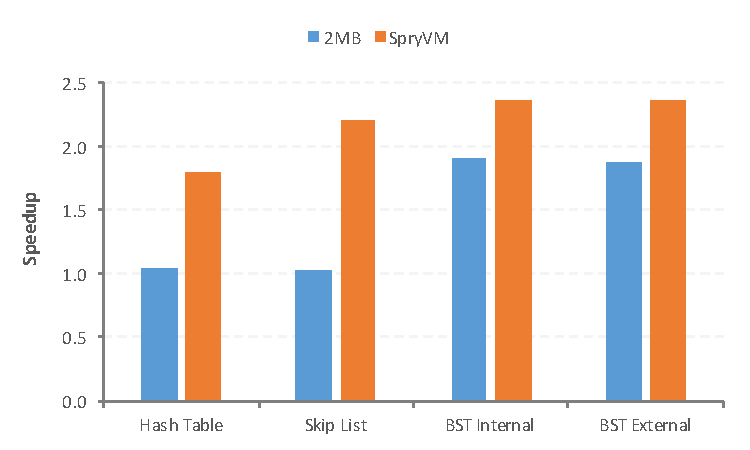
\includegraphics[width=0.25\textwidth,clip]{graphs/speedup_128GB.pdf}}

	\caption{Speedup of conventional translation with $2$MB pages and DTRIM, with respect to conventional $4$KB pages.
		\label{fig:perf}}
\end{figure}

\subsection{Performance}

Figure~\ref{fig:perf} compares the performance of $2$MB pages and DTRIM, with respect to a conventional translation mechanism using $4$KB pages, for $32$GB and $128$GB cases. DTRIM clearly outperforms $4$KB pages in both working set scenarios, by up to $1.8\times$ with $32$GB and $1.7\times$ on average. Furthermore, in $128$GB scenarios, DTRIM outperforms $4$KB pages by up to $2.36\times$ and $2.18\times$ on average. Compared to conventional translation with $2$MB pages, DTRIM outperforms it by up to $1.7\times$ and $1.2\times$ on average for $32$GBs, and by up to $2.15\times$ and $1.6\times$ on average for $128$GB. Furthermore, there is no case in which $2$MB pages outperforms DTRIM in the large-memory scenario.

